%-*-coding: utf-8-*-
\chapter{ 
Параллельные модификации алгоритмов поиска кратчайших путей}

В этой главе будет приведены параллельные модификации алгоритмов поиска кратчайших путей. В начале главы будут предложены модификации алгорима Беллмана-Форда. Во второй части будут приведены два параллельных решения для поиска кратчайших расстояний между каждой парой вершин, а после будет приведено решение задачи для графов социальных сетей.

\FloatBarrier
\section{Параллельный алгоритм Беллмана-Форда}\label{bf_par_secion}

В предыдущей главе были рассмотрены классические алгоритмы поиска кратчайших путей в графе, а также существующие параллельные модификации. В этом разделе будут рассмотрены мною разработанные версии алгоритма Беллмана-Форда в контексте параллельных вычислений. Кроме того, будем использовать в каждом из алгоритмов идею ранней остановки --- если на текущем шаге ни одно из значений массива расстояний не изменилось, то имеем право выйти из основного цикла. 

\FloatBarrier
\subsection{Параллелизация по ребрам вершины}

Прежде чем приступить к описанию параллельной версий выполним небольшую модификацию алгоритма. Будем для каждой вершины перебирать не исходящие ребра, а входящие. Это ход даст нам одно важное преимущество в контексте параллельных алгоритмов --- значение кратчайшего расстояния до каждой вершины теперь может изменять лишь один поток, тогда как раньше могли несколько, что увеличивало потенциальные проблемы с гонками за ресурс.

\begin{figure}[h]
\centering
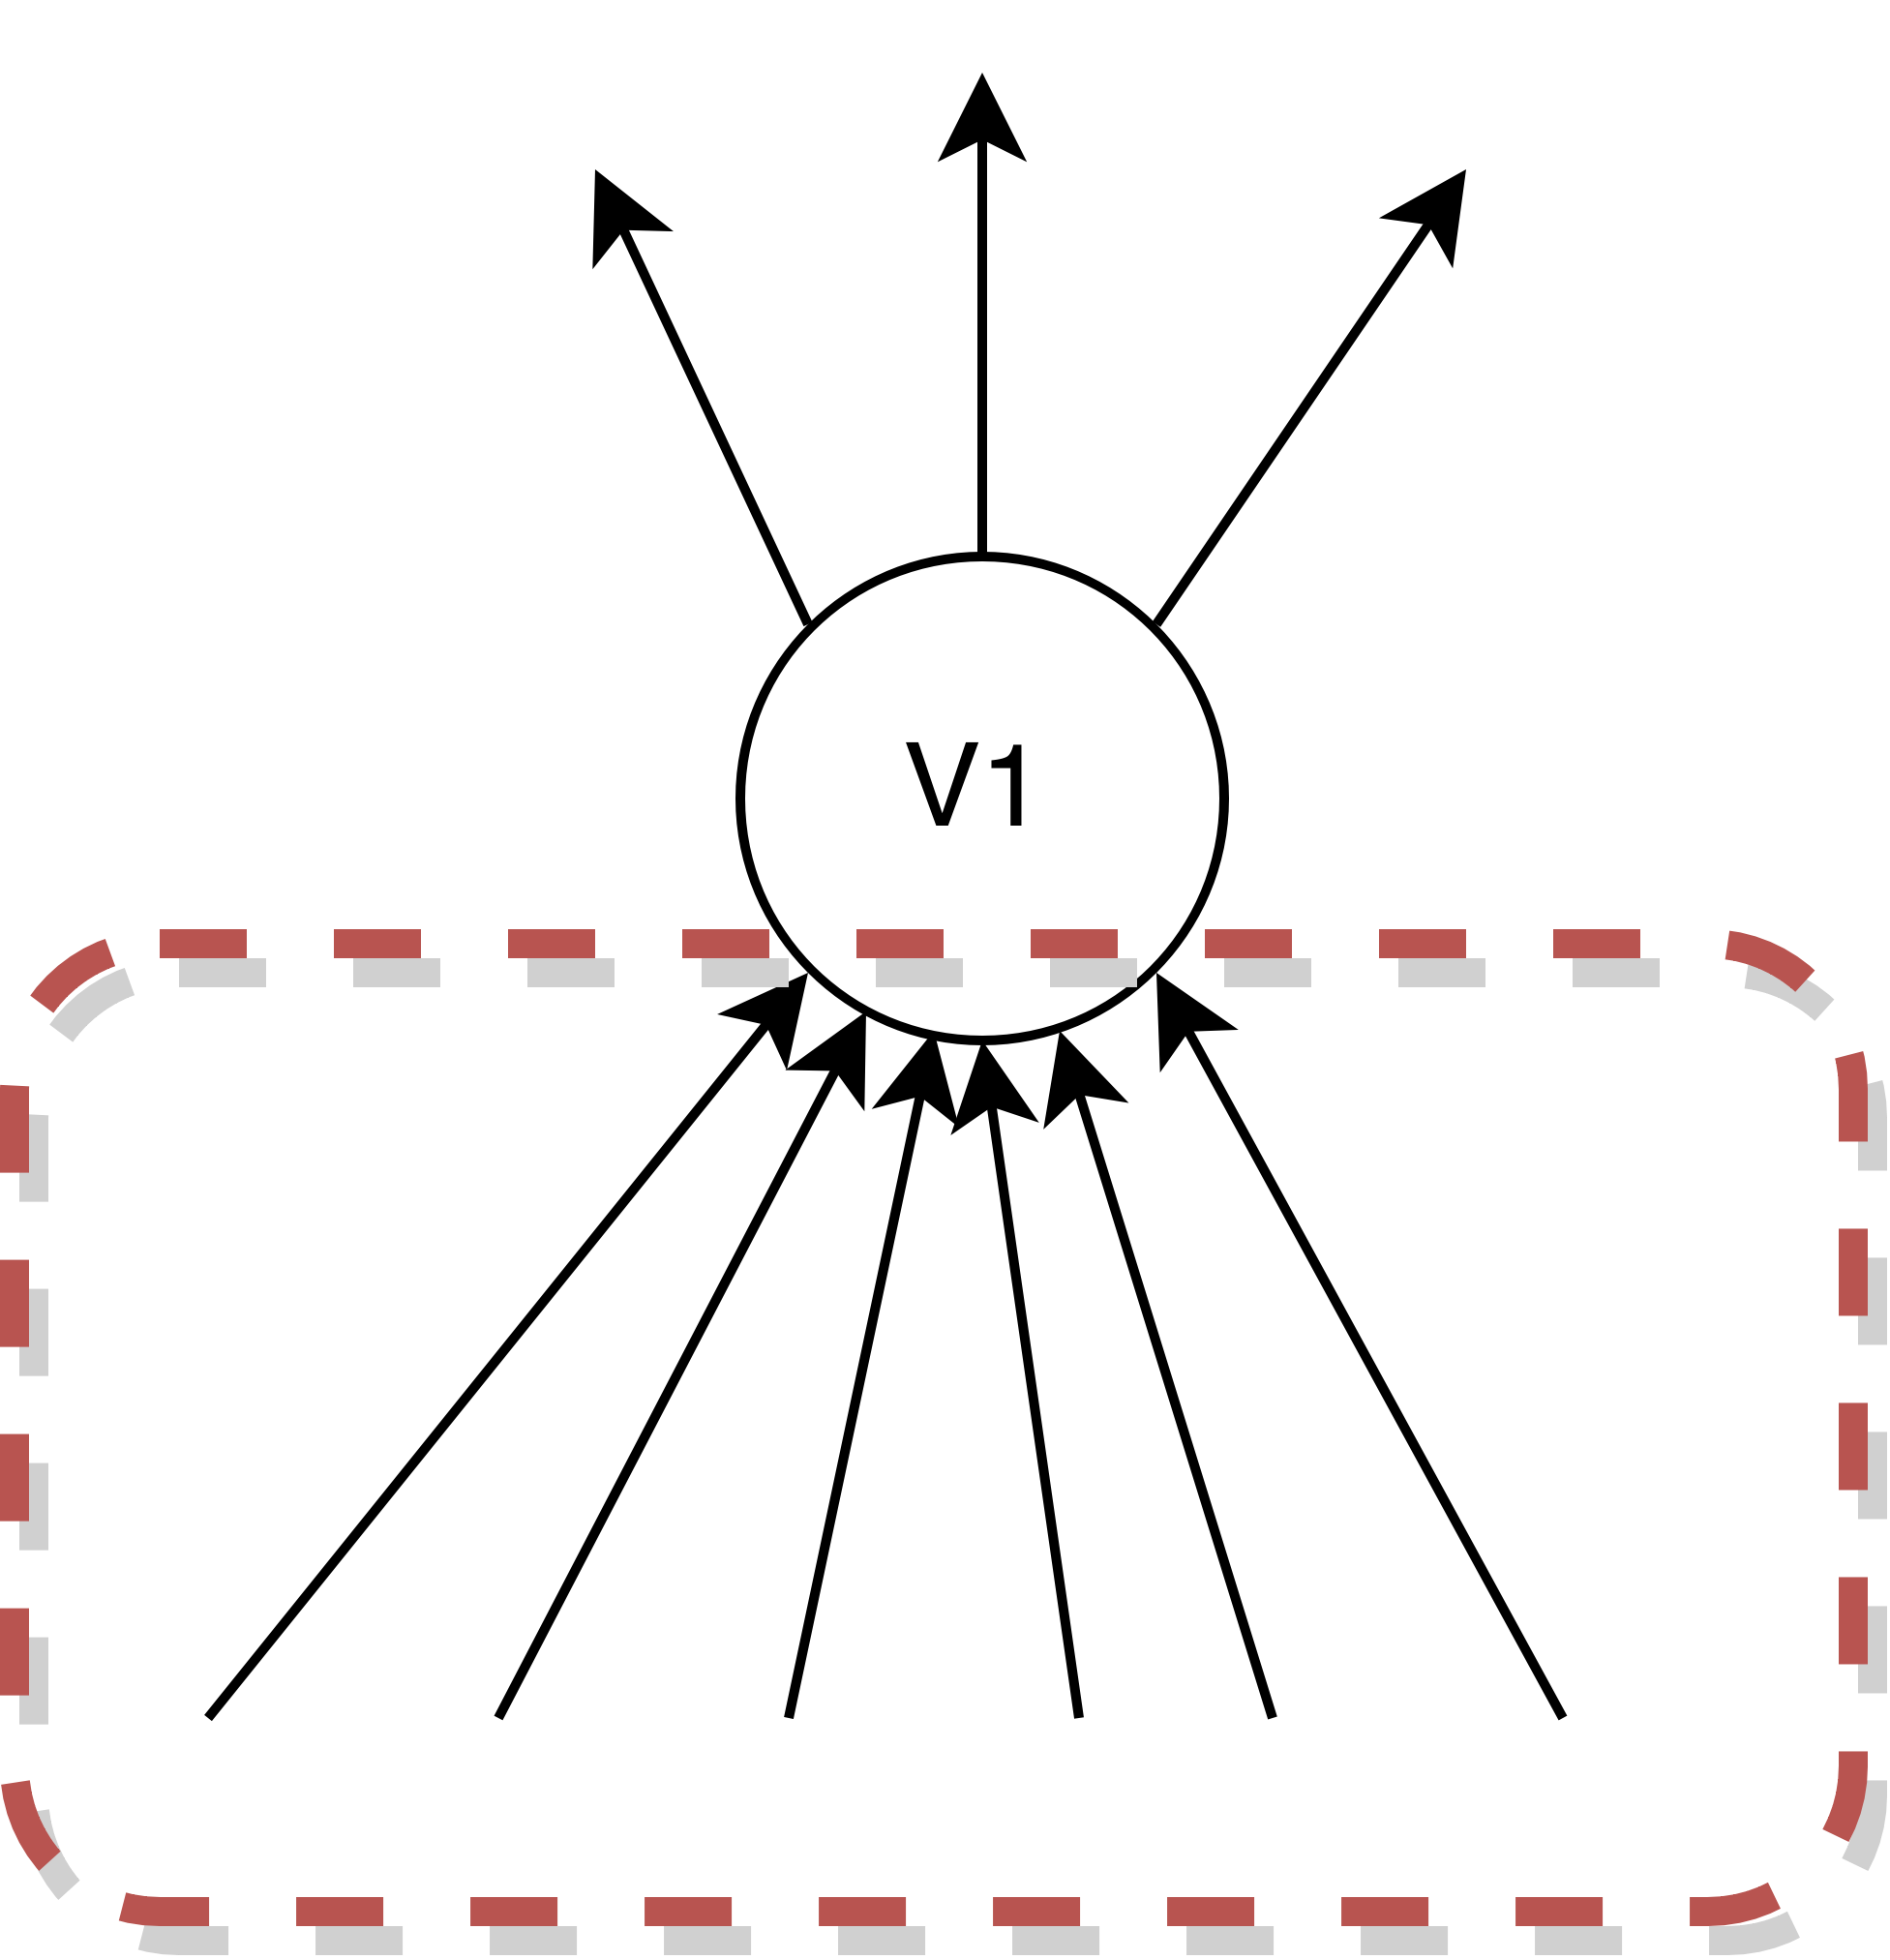
\includegraphics[width=0.4\textwidth]{img/bf_par_1.png}
\caption{Параллелизация по ребрам вершины}
\label{bf_par_1}
\end{figure}

Первая версия алгоритма основана на параллельной обработке всех ребер, входящих в текущую вершины. Псевдокод, который уже использует идею из предыдущего абзаца, приведен ниже. Алгоритм, как и классическая версия, работает в худшем случае за $O(VE)$. 



\FloatBarrier
\begin{algorithm}
\caption{Параллельный Беллман-Форд по ребрам вершины}\label{bf_classic_par1}
\begin{algorithmic}[1]
\Procedure{BellmanFordPar1}{$G,start$}
\State $dist\gets \left\{ {\infty ... \infty}\right\}$
\State $dist[start] \gets 0$
 
\For{$i = 0$ to $|G.vertices| - 1 $}
	\State {$changed \gets $ \algorithmicfalse}
	\For{$v \in G.vertices $}
		\algrenewcommand\algorithmicfor{\textbf{parfor}}
		\State $minDist \gets dist[v]$

		\For{$e \in G.edgesTo[v] $} \Comment{Входящие ребра в текущую вершину} 
			\State $minDist \gets \min(minDist, dist[e.from] + e.w)$
		\EndFor	
					
		\If {$dist[v] > minDist$} 
			\State $dist[v] \gets minDist$ \Comment{Атомарно} 

			\State {$changed \gets $ \algorithmictrue}					
		\EndIf

		\algrenewcommand\algorithmicfor{\textbf{for}}

	\EndFor
	\If {\algorithmicnot $changed$} 
		\State \textbf{break}
	\EndIf

\EndFor
\State \textbf{return} $dist$
\EndProcedure
\end{algorithmic}
\end{algorithm}
\FloatBarrier



\FloatBarrier
\subsection{Параллелизация по всем ребрам}
Идея второго алгоритма состоит в разбиений всего набора вершин на некоторые подмножества, каждое из которых будет обрабатываться отдельным процессором. При этом опять же, как и в предыдущем алгоритме, для каждой вершины будем рассматривать набор ребер, входящих в нее. 

Рассмотрим псеводкод алгоритма. Процесс поиска расстояний разбивается на два этапа. Рассмотрим каждый из этапов по отдельности.

На первом этапе мы строим разбиение всего множества вершин на подмножества, каждое из которых будет обрабатываться последовательно. Причем необходимо выполнить разбиение таким образом, чтобы суммарное количество входящих в вершины текущего подмножества ребер было не более $threshold$. Добиться этого можно с помощью рекурсивной функции $BuildPlan$, которая на текущем шаге находит с помощью двоичного поиска такую вершину текущего отрезка, которая разбивает множество входящих в вершины ребер примерно пополам. Далее индекс такой вершины запоминается в хэш-таблицу, ключом которой является пара индексов концов текущего отрезка. Для эффективной реализации двоичного поиска предпосчитаем частичные суммы для входящих ребер --- это необходимо, чтобы мы могли в двоичном поиске получать за $O(1)$ количество входящих ребер на некотором отрезке вершин. 

\FloatBarrier


На втором этапе мы непосредственно вычисляем кратчайшие расстояния до вершин. Эта функция использует посчитанные раннее частичные суммы и полученную из функции $BuildPlan$ хэш-таблицу. На текущем шаге функция проверяет больше ли количество входящих ребер текущего отрезка значения $threshold$. Если значение оказывается меньше, то обработка ребер выполняется последовательно. Иначе, с помощью посчитанной на первом этапе хэш-таблицы выбирается индекс середины отрезка (в смысле числа входящих ребер) и параллельно запускается обработка двух подотрезков вершин. Операция выбора середины отрезка будет выполняться за $O(1)$ за счет хэш-таблицы.

\FloatBarrier
\begin{algorithm}[H]
\caption{Параллельный Беллман-Форд по всем ребрам}\label{bf_classic_par2}
\begin{algorithmic}[1]
\Procedure{BellmanFordPar2}{$G,start$}
\State $dist\gets \left\{ {\infty ... \infty}\right\}$
\State $dist[start] \gets 0$
\State {$prefsum \gets $ prefix sum by vertices incoming degree} 
\State {$planMap \gets $ empty map}
\State \Call {BuildPlan}{$prefsum$, 0, |$G.vertices$|, planMap}

\For{$i = 0$ to $|G.vertices| $}	
	\If {\algorithmicnot \Call {ProcessLayer}{$G, dist, planMap, prefsum, 0, |G.vertices|$}} 
		\State \textbf{break}
	\EndIf
		
\EndFor
\State \textbf{return} $dist$
\EndProcedure

\State 
\Procedure{BuildPlan}{$prefsum, startV, endV, resultMap$}  
\State $edgesNumber \gets prefsum[endV] - prefsum[startV]$
\If {$edgesNumber < threshold$} 
	\State $midV \gets $ Бинарным поиском по массиву prefsum находим индекс вершины $midV$, что $prefsum[midV]-prefsum[startV] \approx prefsum[endV]-prefsum[midV]$
	\State $resultMap[startV][endV] \gets midV$ 
	\State \Call {BuildPlan}{$prefsum, startV, midV, resultMap$} 
	\State {\Call {BuildPlan}{$prefsum, midV, endV, resultMap$}} 
\EndIf

\State \textbf{return} $resultMap$
\EndProcedure

\State 
\Procedure{ProcessLayer}{$G, dist, planMap, prefsum, startV, endV$}  
\State $edgesNumber \gets prefsum[endV] - prefsum[startV]$
\If {$edgesNumber < threshold$} 
	\State {\textbf{return} {\Call {ProcessVerticesSequentially}{$G, dist, startV, endV$}}}
\Else	
	\State $midV \gets planMap[startV][endV]$ 
	\State {$changed \gets $ \algorithmicfalse}

	\State {$changed = changed $ \algorithmicor \Call {ProcessLayer}{$G, dist, planMap, prefsum, startV, midV$}}
	\State {$changed = changed $ \algorithmicor \Call {ProcessLayer}{$G, dist, planMap, prefsum, midV, endV$}}
	\State \textbf{return} $changed$
\EndIf

\EndProcedure

\State 
\Procedure{ProcessVerticesSequentially}{$G, dist, startV, endV$}  

\State {$changed \gets $ \algorithmicfalse}
\For{$v = startV$ to $endV - 1 $}
		\State $minDist \gets dist[v]$

		\For{$e \in G.edgesTo[v] $} \Comment{Входящие ребра в текущую вершину} 
			\State $minDist \gets \min(minDist, dist[e.from] + e.w)$
		\EndFor	
					
		\If {$dist[v] > minDist$} 
			\State $dist[v] \gets minDist$ \Comment{Атомарно} 

			\State {$changed \gets $ \algorithmictrue}					
		\EndIf
\EndFor
\State \textbf{return} $changed$

\EndProcedure

\end{algorithmic}
\end{algorithm}

\begin{figure}[h]
\centering
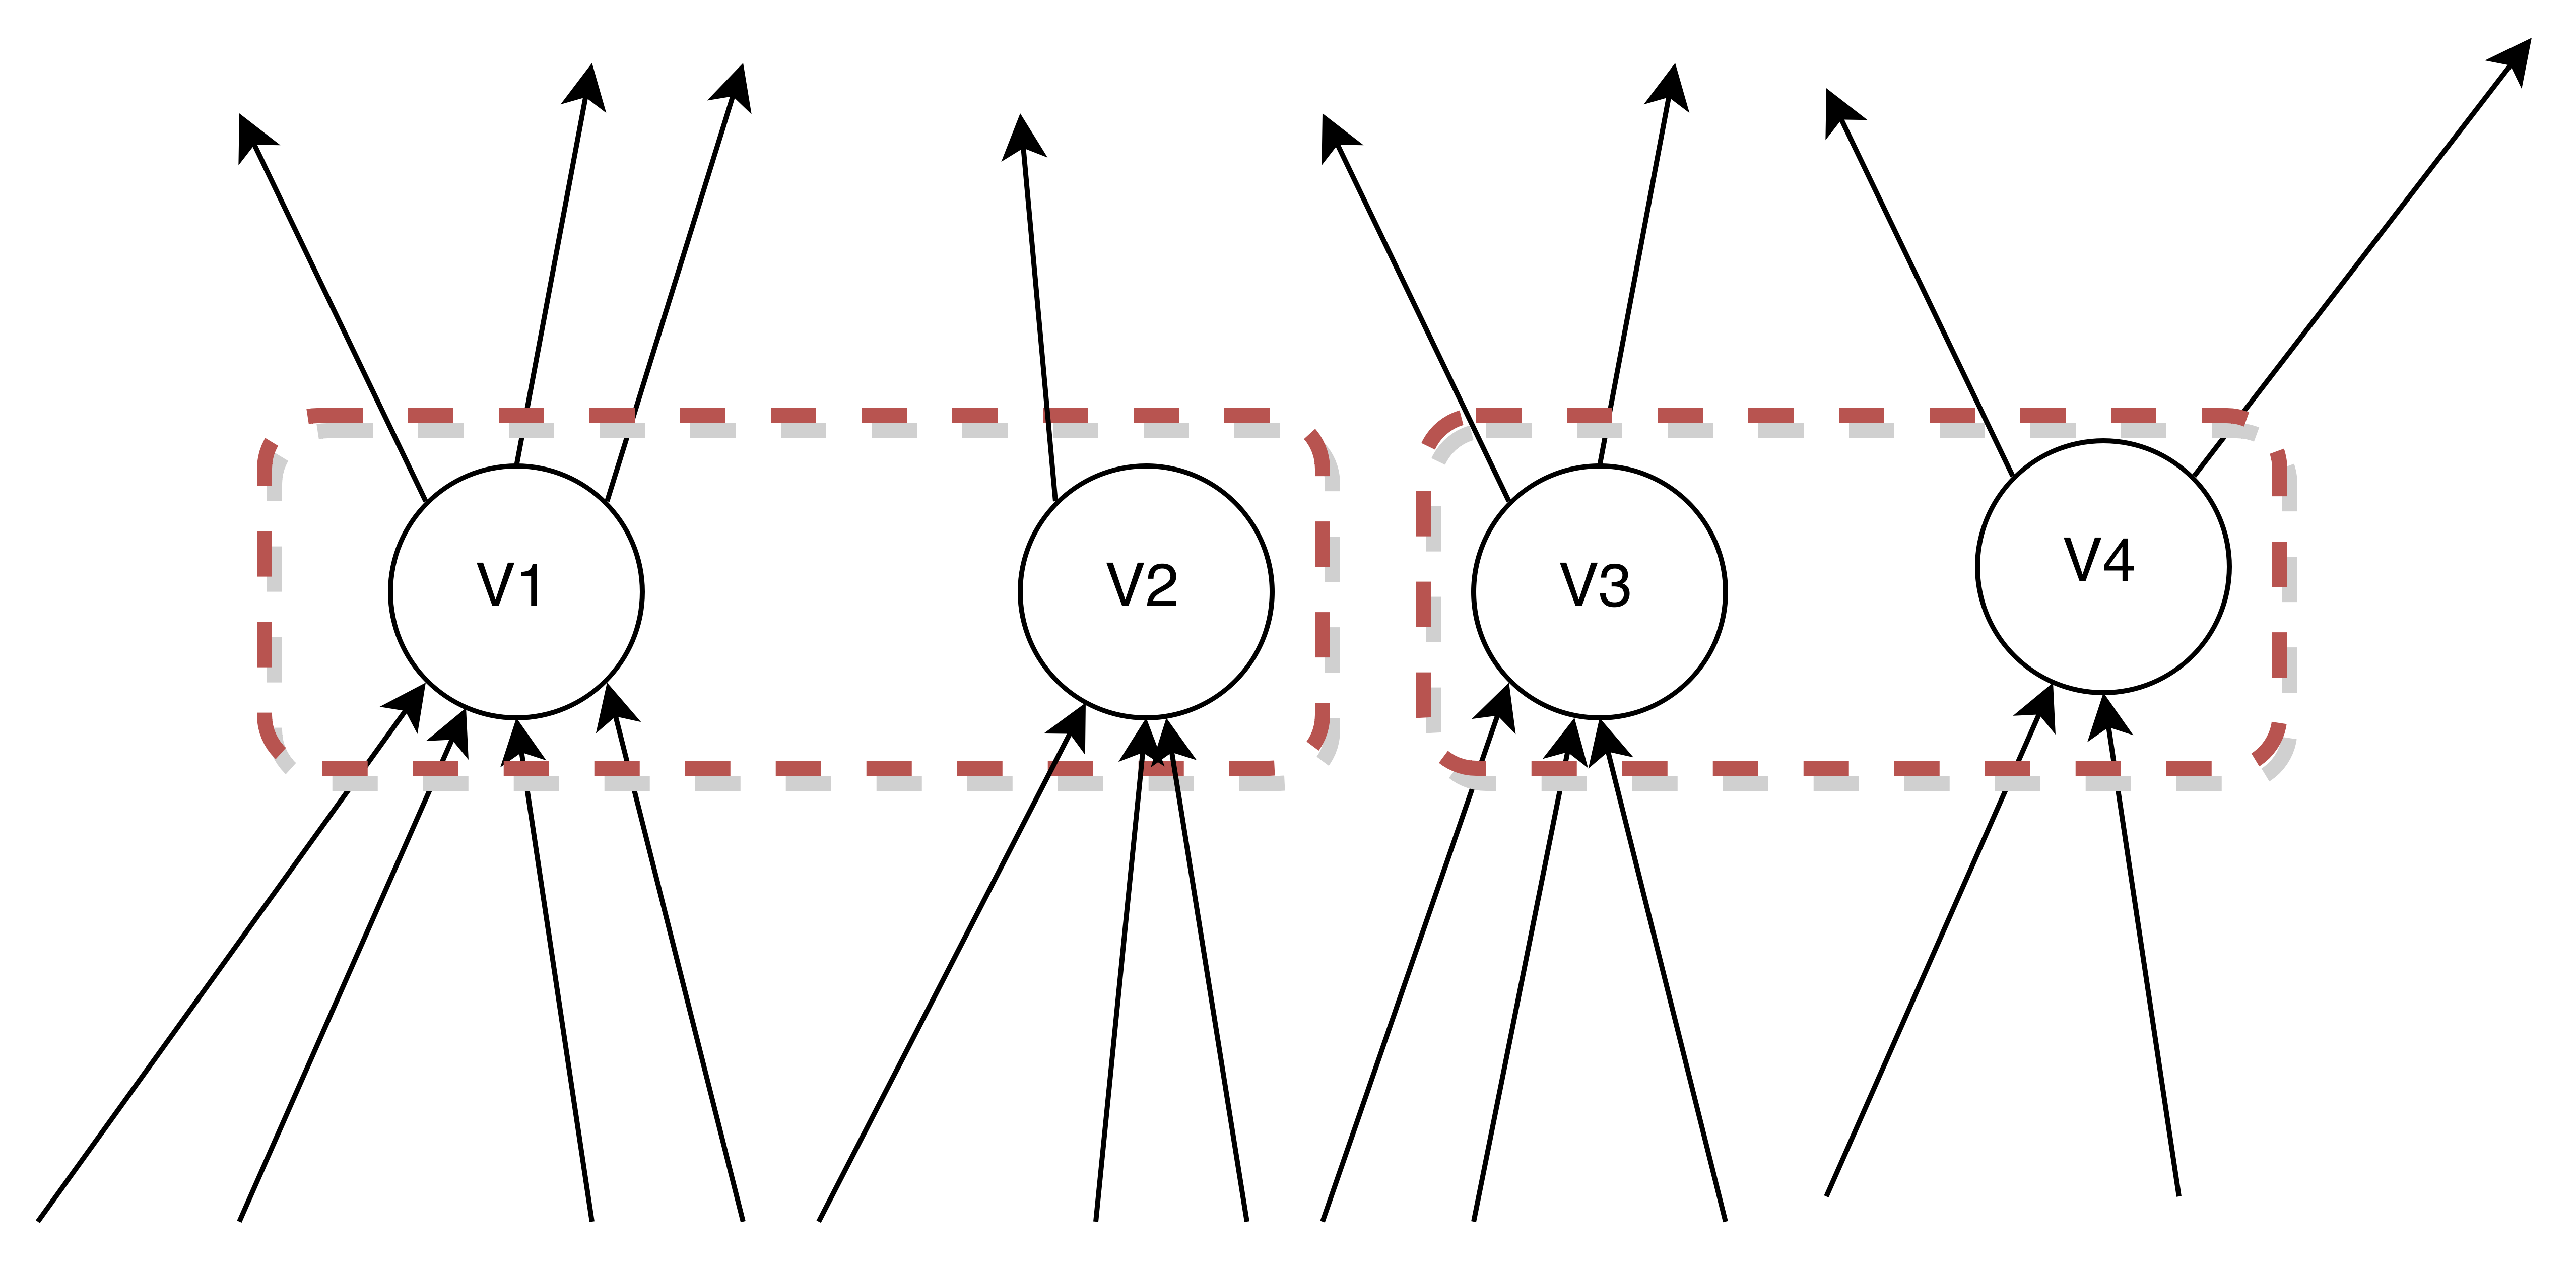
\includegraphics[width=0.8\textwidth]{img/bf_par_2_2.png}
\caption{Параллелизация по всем ребрам}
\label{bf_par_2_2}
\end{figure}


Алгоритм также как и предыдущая версия работает в худшем случае за $O(VE)$, однако он имеет значительно большую практическую пользу. Эта тема будет подробно рассмотрена позднее в главе, посвященной сравнению подходов.


\FloatBarrier
\subsection{Параллелизация BFS-версии}
Предыдущие две версии были основаны на параллелизации классической версии Беллмана-Форда. В основе следующего алгоритма лежит BFS-подобный Беллман-Форд (алгоритм \ref{bf_bfs_seq}). В качестве основы для параллельной версии такого алгоритма был взят параллельный обход в ширину, предложенный Умутом Акаром и Майком Рэйни \cite{FRONTIERSEARCH}. 


Ключевым моментом в алгоритме является использованием структуры данных Frontier. Она подробно рассмотрена в статье Умута Акара и Майка Рэйни. Здесь же приведено краткое ее описание, основные принципы работы и интерфейс. Frontier представляет из себя некоторый набор ребер. При этом он поддерживает операции разделения множества пополам, слияния множеств, добавления ребер вершины и итерирования по ребрам. При этом  операции слияния и разбиения выполняются асимптотически за $O(\log n)$, добавление ребер вершины происходит за константу, а итерирование за константу для каждого ребра. Такая асимптотика достигается за счет лежащей в основе Bootstrapped Chunked Sequence \cite{CHUNKEDSEQ}, которая представляет из себя последовательность, где каждому элементу сопоставляется его вес. И операций слияния и разбиения выполняются в соответсвии с этими весами и выполняются за $O(\log n)$. Более подробное описание Bootstrapped Chunked Sequence приведено в указанной раннее статье. 

\begin{figure}[h]
\centering
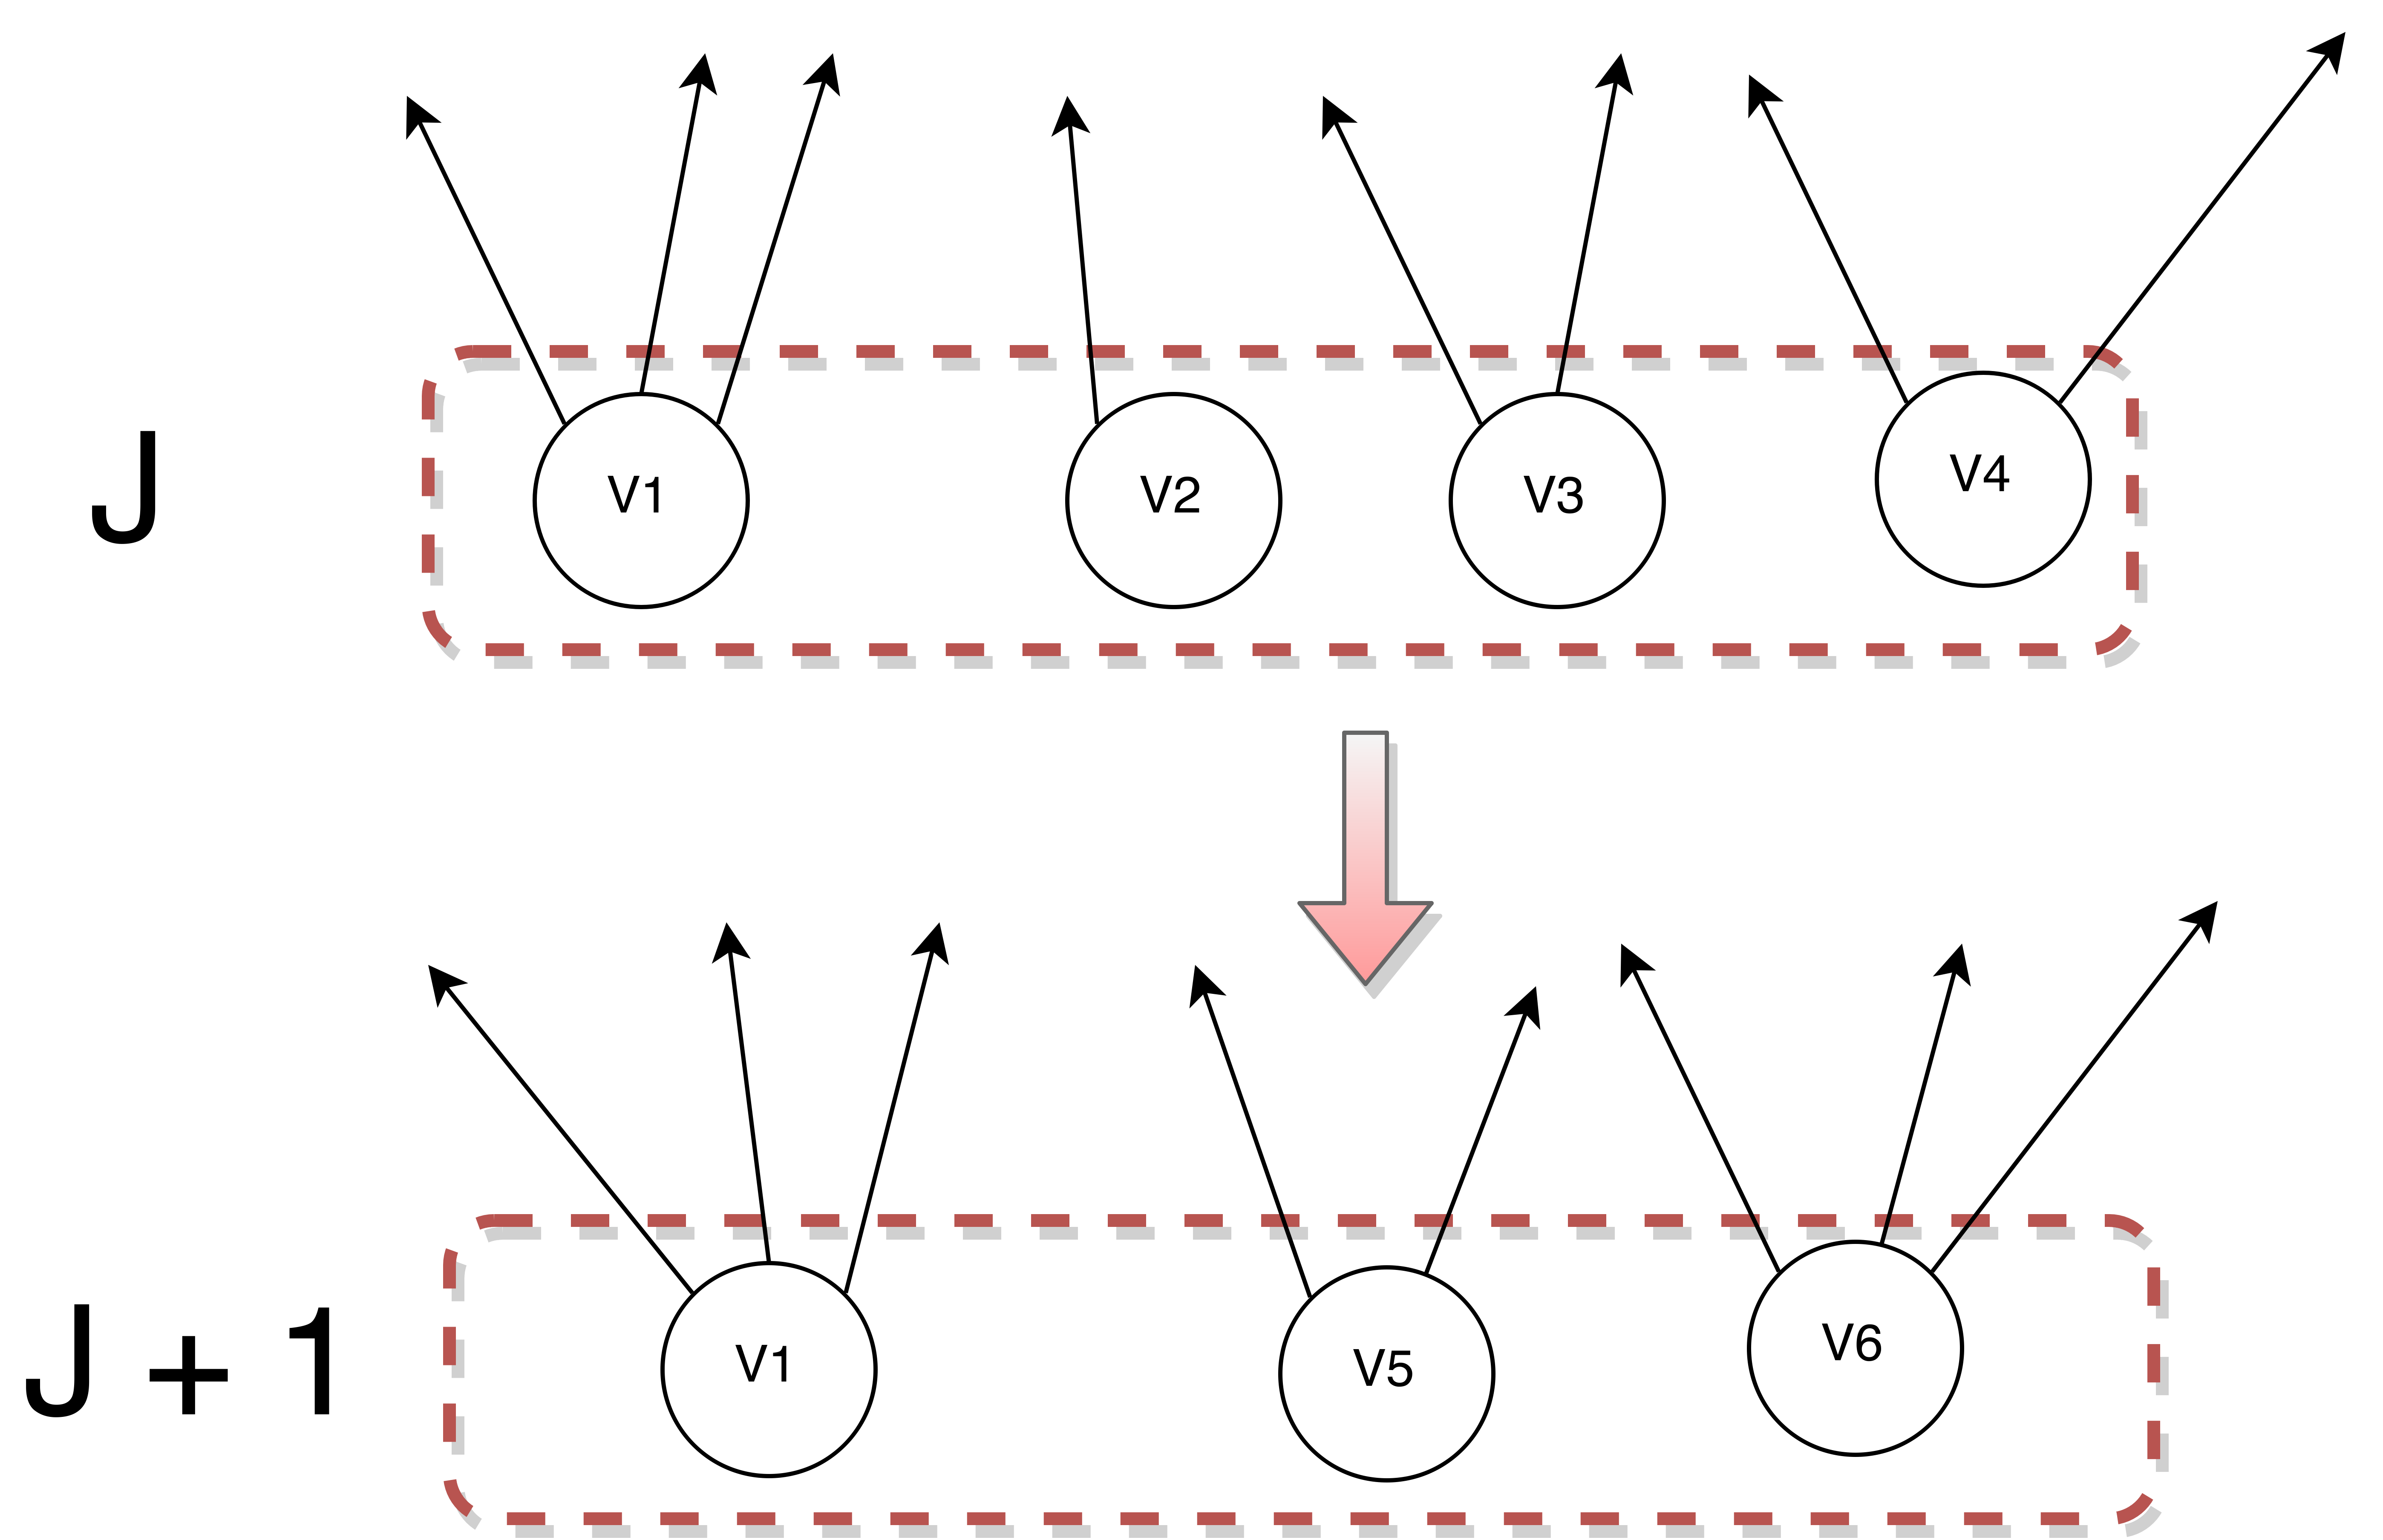
\includegraphics[width=0.75\textwidth]{img/bf_par_3.png}
\caption{Параллелизация BFS-версии}
\label{bf_par_3}
\end{figure}

Кроме того, в алгоритме используются важная возможность библиотеки для параллельных вычислений PASL \cite{PASL} (является альтернативой известного решения Cilk \cite{CILK}) --- взаимодействие между несколькими потоками. А именно каждый из потоков может понимать нуждаются ли в «помощи» другие потоки. И в случае положительного ответа он может «поделиться» данными для вычислений. 

Таким образом, псевдокод алгоритма представлен ниже. В основе главной функции алгоритма $HandleFrontier$ лежит следующая идея. В процессе обработки текущего $CurFrontier$ мы во-первых узнаем нуждается ли другой процессор в данных для вычисления. Если да, то делимся в случае достаточного количества ребер. Иначе обрабатываем некоторое константное значение ребер ($pollingCutoff$) и запускаем процесс снова. Обратим внимание, что в нем использованы упомянутые ранее возможности библиотеки PASL --- функции $hasIncomingQuery$ и $rejectQuery$. 



\begin{algorithm}[H]
\caption{Параллельный BFS-подобный Беллман-Форд}\label{bf_bfs_par}
\begin{algorithmic}[1]
\Procedure{BellmanFordPar3}{$G,start$}
\State $dist\gets \left\{ {\infty ... \infty}\right\}$
\State $layerForVertex\gets \left\{ {-1 ... -1}\right\}$ \Comment{Номер последнего уровня, в котором посетили вершину} 
\State $dist[start] \gets 0$
\State $layerForVertex[start] \gets 0$
\State {$Frontier \gets \left\{ {G.edgesFrom(start)}\right\}$}\Comment{Исходящие ребра текущего множества } 

\For{$layer = 1$ to $|G.vertices| $}	
	\State $NextFrontier \gets \emptyset$

	\State {$Frontier \gets $  {\Call {HandleFrontier}{$Frontier, NextFrontier, layer, dists, layerForVertex$}}} 
	
	\If { $Frontier.empty()$} 
		\State \textbf{break}						
	\EndIf
		
		
\EndFor
\State \textbf{return} $dist$
\EndProcedure
\State

\Procedure{HandleFrontier}{$CurFrontier, NextFrontier, layer, dists, layerForVertex$}
\While {\algorithmicnot $CurFrontier.empty()$}
	\If {$hasIncomingQuery()$}
		\If {$CurFrontier.nbEdges() \leq cutoff$}
			\State $rejectQuery()$			
		\Else		
			\State $NewCurFrontier \gets \emptyset$
			\State $NewNextFrontier \gets \emptyset$
			\State $CurFrontier.split(NewCurFrontier)$
			\State \begin{varwidth}[t]{\linewidth}fork2(\par
        \hskip\algorithmicindent {\Call {HandleFrontier}{$CurFrontier, NextFrontier, layer, dists, layerForVertex$}},\par
        \hskip\algorithmicindent {\Call {HandleFrontier}{$NewCurFrontier, NewNextFrontier, layer, dists, layerForVertex$}});
      \end{varwidth}
 			\State $NextFrontier.split(NewNextFrontier)$

		\EndIf
		
	\EndIf
	\State Frontier.iterNumber(pollingCutoff, updateFunction(from, to, weight, layer, dists, layerForVertex))
\EndWhile
\EndProcedure
\State
\Procedure{UpdateFunction}{$from, to, weight, layer, dists, layerForVertex, NextFrontier$}
\If {{\Call {TryToUpdateDistance}{$to, dists[from] + weight, dists$}}} 

	\If {{\Call {TryToSetVisited}{$to, layer, layerForVertex$}}} 
		\State $NextFrontier.pushEdgesOf(to)$
	\EndIf
	
\EndIf
\EndProcedure
\State
\Procedure{TryToSetVisited}{$vertex, layer, layerForVertex$}
\If {\algorithmicnot $layerForVertex[vertex] = layer$} 
	\State \textbf{return} {$cas(layerForVertex[vertex], layerForVertex[vertex], layer)$ }  
\EndIf
\State \textbf{return} {\algorithmicfalse}  
\EndProcedure
\State
\Procedure{TryToUpdateDistance}{$vertex, candidate, dists$}
\State \textbf{return} {$writeMin(dists[vertex], candidate)$} \Comment Атомарный минимум 
\EndProcedure

\end{algorithmic}
\end{algorithm}



\FloatBarrier


\FloatBarrier
\section{Параллельные алгоритмы поиска кратчайших расстояний между каждой парой вершин}\label{floyd_par_secion}

В данном разделе представлены мною разработанные параллельные версии алгоритмов для поиска кратчайших расстояний между каждой парой вершин --- наивная параллельная версия, модификация для объединенных графов и эффективный алгоритм для решения поставленной задачи на невзвешенных и неориентированных графах реальных социальных сетей.

\FloatBarrier
\subsection{Наивная параллельная версия}
Первая версия заключается исключительно в запуске параллельного Беллмана-Форда для каждой из вершин. При этом заметим, что так как каждый из них независим друг от друга, то можем эти запуски распараллелить между собой. Для этого разобьем множество вершин таким образом, чтобы размер каждого подмножества был не более $threshold$. Важным замечанием является то, что необходимо выбирать наиболее подходящую реализацию параллельного Беллмана-Форда в зависимости от типа графа. К примеру, в случае разреженного графа с положительными ребрами нам подойдет последняя реализация, основанная на параллельном обходе в ширину. Таким образом, псевдокод из себя представляет следующее.


\FloatBarrier
\begin{algorithm}
\caption{Наивная параллельная версия}\label{all_pairs_par1}
\begin{algorithmic}[1]
\Procedure{AllPairsPar1}{$G$}
\State \textbf{return} {\Call {HandleVertices}{$G, 0, |G.vertices|$}}
\EndProcedure
\State
\Procedure{HandleVertices}{$G, startVertex, endVertex$}

\If {$endVertex - startVertex < threshold$} 
	\State $distances \gets$ Запустить параллельную версию Беллмана-Форда для каждой вершины из полуинтервала $[startVertex, endVertex)$ 
	\State \textbf{return} $distances$	
\Else	
	\State $midVertex \gets (startVertex + endVertex) / 2$ 
	\State \begin{varwidth}[t]{\linewidth}fork2(\par
        \hskip\algorithmicindent {\Call {HandleVertices}{$G, startVertex, midVertex$}},\par
        \hskip\algorithmicindent {\Call {HandleVertices}{$G, midVertex, endVertex$}});
      \end{varwidth}
	
\EndIf

\EndProcedure

\end{algorithmic}
\end{algorithm}

\FloatBarrier
\subsection{Параллельный алгоритм для объединенного графа}
Развитием предыдущей идеи является наблюдение, что для некоторого набора вершин можем построить общий граф и запустить на нем Беллмана-Форда, что потенциально может повысить производительность за счет больших размеров текущего Frontier в процессе работы алгоритма, ведь маленькие размеры Frontier, которые могут появляться при запуске алгоритма из одной вершины, значительно снижают параллелизм. Кроме того, такой подход избавит нас от выбора константы $threshold$ из предыдущего раздела, что упростит использование алгоритма. 

Идея заключается в запуске алгоритма Беллмана-Форда на графе, каждой вершине которого соответсвует две вершины $i$ и $j$ исходного графа. При этом ребро $(i, j) \rightarrow (k, l)$ в новом графе существует тогда и только тогда, когда существует ребро между вершинами $i$ и $k$ в исходном графе и $j = l$. Пример построения такого графа представлен на рисунке \ref{floyd_par_common_graph}. При этом если мы на получившемся графе одновременно запустим Беллмана-Форда для всех вершин вида $(i, i)$ (положим все вершины такого вида в изначальный Frontier), то найденное кратчайшее расстояние до некоторой вершины $(i, j)$ будет интерпретироваться как кратчайшее расстояние от вершины $i$ до вершины $j$ в исходном графе. 
\FloatBarrier
\begin{figure}[h]
\centering
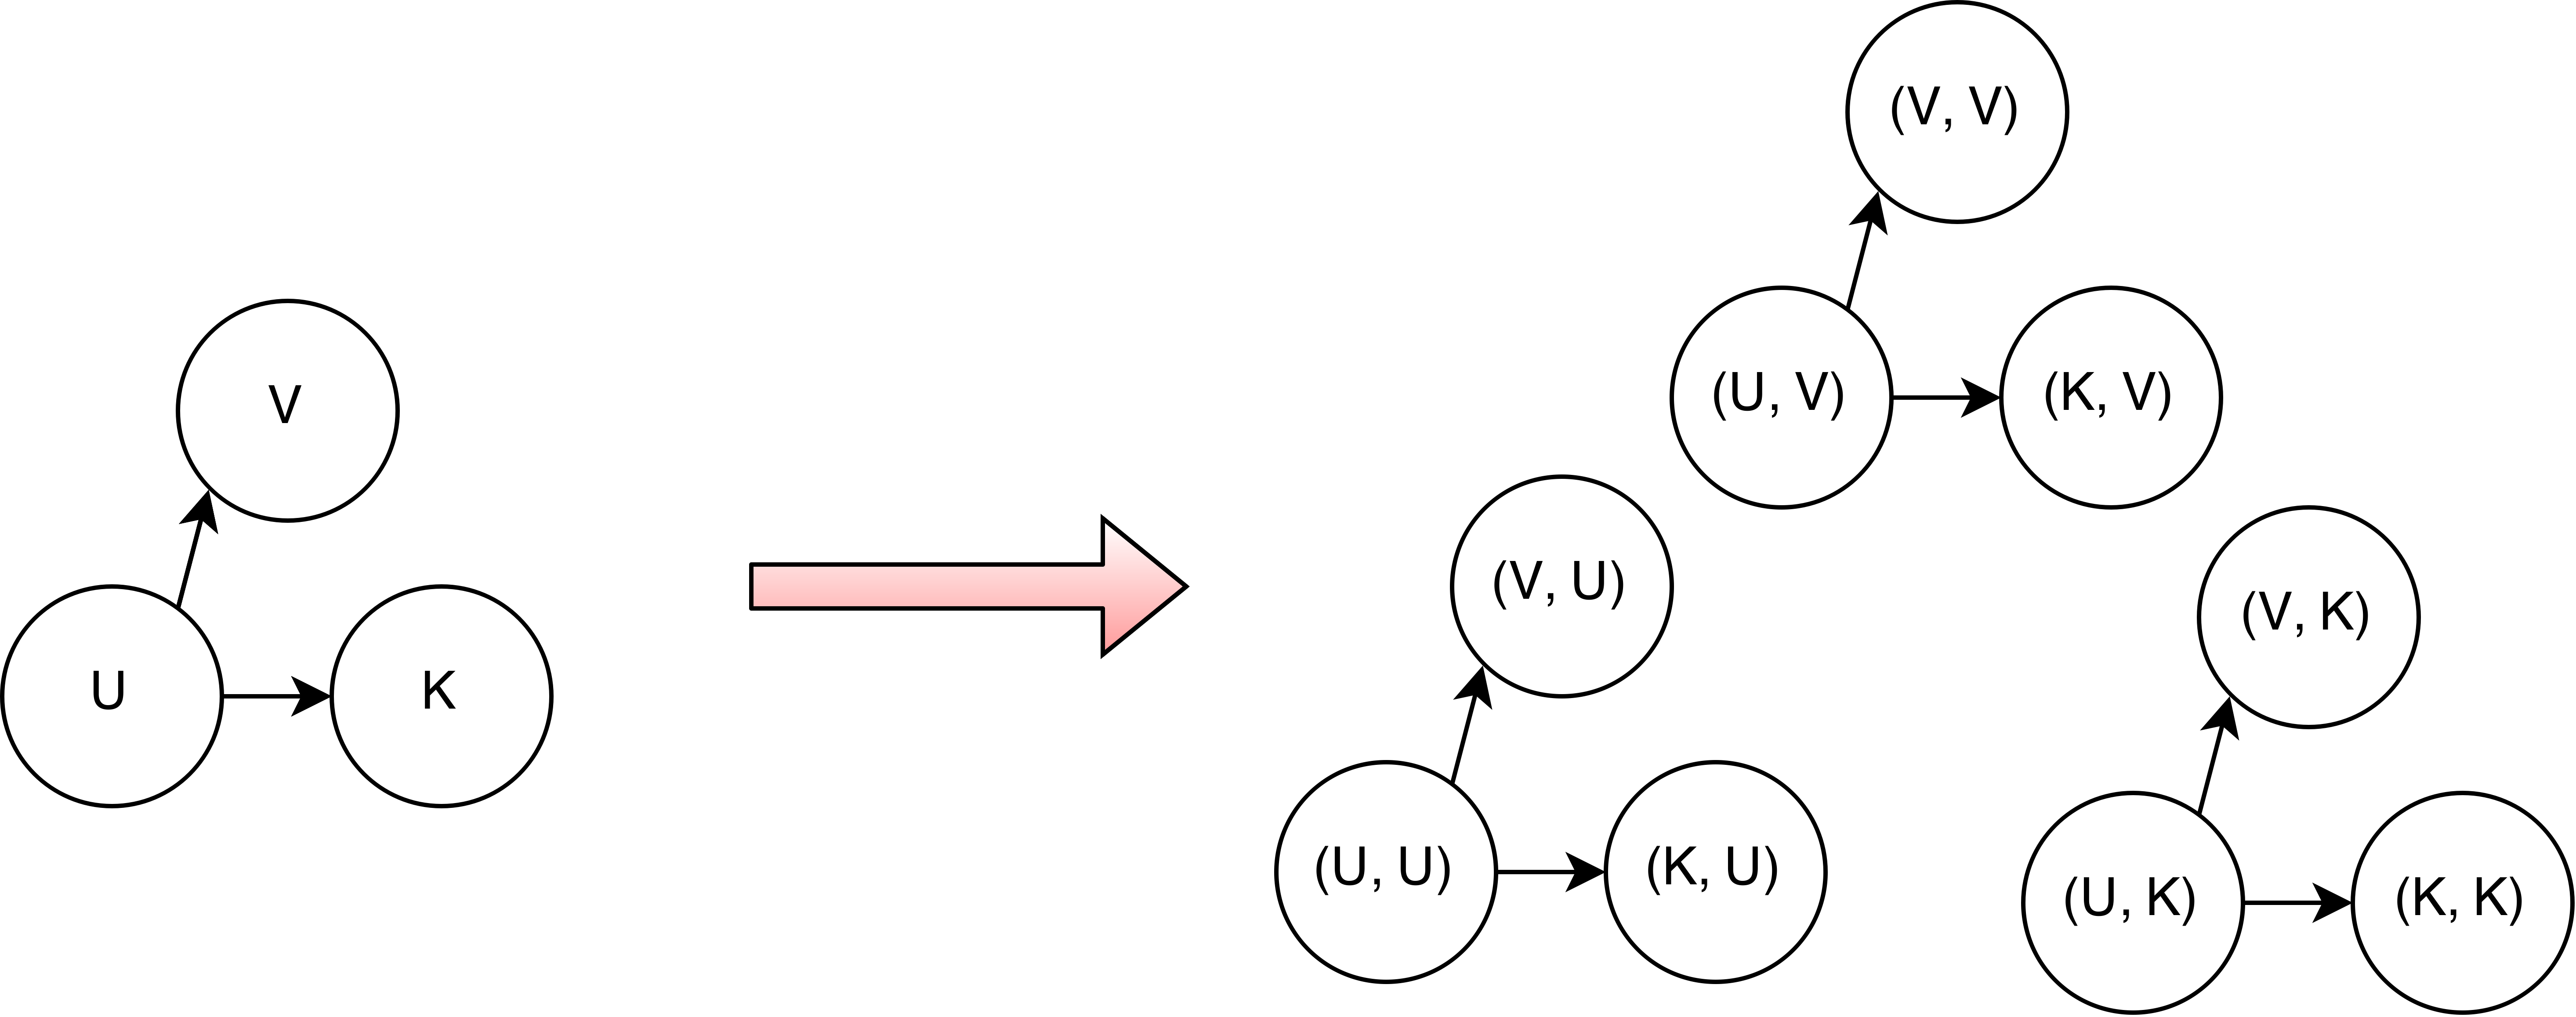
\includegraphics[width=0.9\textwidth]{img/floyd_par_2.png}
\caption{Пример преобразования для простейшего графа}
\label {floyd_par_common_graph}
\end{figure}
\FloatBarrier

Однако, как было показано на практике, такой подход не дал существенного выигрыша в силу высокой параллельности наивного метода, но при этом идея обработки ряда вершин одновременно легла в основу алгоритма для социальных графов. 

\FloatBarrier
\subsection{Параллельный алгоритм для социальных графов}
В данном подразделе описана идея, принцип работы и модификация параллельного алгоритма поиска кратчайших расстояний между каждой парой вершин в невзвешенных и неориентированных графах реальных социальных сетей.
\FloatBarrier
\subsubsection{Идея алгоритма}
В графах для социальных сетей известна одна эвристика, которая называется «Теория шести рукопожатий». В ее основе лежит тот факт, что практически любые два человека на земле знакомы не более, чем через пятерых промежуточных людей. Таким образом, выбрав некоторую случайную вершину, мы сможем добраться от нее до большинства других вершин не более, чем за 6 ребер. Воспользуемся этой эвристикой в нашем алгоритме и выберем вершину наибольшей степени в качестве базовой. И рассмотрим два множества --- вершины, которые находятся на расстоянии не более 6 от базовой («большее» множество) и все остальные вершины («меньшее» множество). Кроме того, будем обрабатывать эти два множества различным образом --- для меньшего будем запускать параллельного Беллмана-Форда для каждой вершины, для большого --- воспользуемся методом динамического программирования для подсчета ответа. Пример разбиения социального графа на два эти множества проиллюстрирован на рисунке \ref{floyd_social}. Рассмотрим более подробно принцип работы алгоритма.

\FloatBarrier
\subsubsection{Работа алгоритма}
Как уже было отмечено ранее, работа алгоритма разбивается на три этапа, которые в дальнейшем будут рассмотрены по отдельности.

\begin{itemize}
  \item Анализ графа и выбор базовой вершины; 
  \item Обработка меньшего множества параллельным Беллманом-Фордом;
  \item Обработка большего множества методом динамического программирования.
\end{itemize}


\begin{figure}[h]
\centering
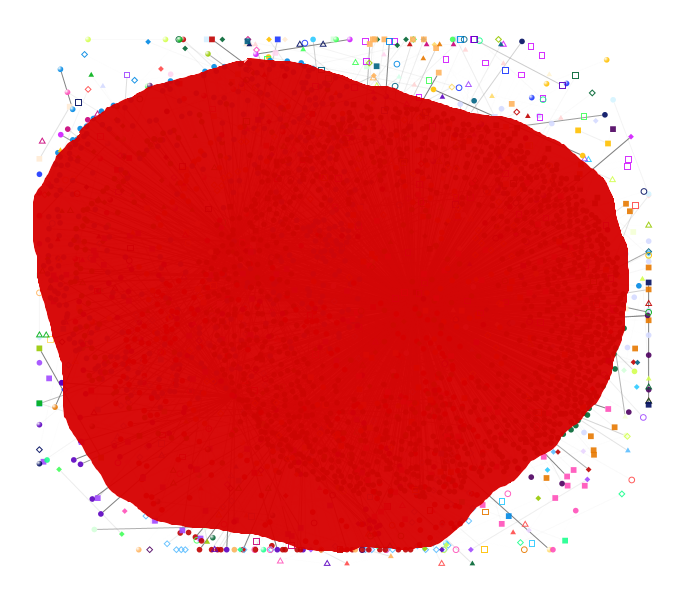
\includegraphics[width=0.9\textwidth]{img/floyd_social.png}
\caption{Пример разбиение социального графа на 2 множества}
\label {floyd_social}
\end{figure}

Первый и самый простой этап состоит в выборе базовой вершины. В качестве нее будет выбрана вершина с наибольшей степенью. После этого из этой вершины будет запущен обход в ширину, который найдет все вершины, отстоящие не более, чем на $K$ (в случае классической теорий шести рукопожатий $K = 6$). Таким образом, все такие вершины попадают в большее множество $handleByBaseVertexSet$, которое будет обработано на третьем этапе алгоритма. Все остальные вершины попадают в меньшее множество $otherVertexSet$. Псевдокод этого этапа выглядит следующим образом.

\FloatBarrier
\begin{algorithm}
\caption{Первая фаза алгоритма}\label{all_pairs_social1}
\begin{algorithmic}[1]
\Procedure{ConstructSets}{$G$}
\State {$baseVertex \gets $ Вершина максимальной степени}
\State {$dist \gets $ Запустить обход в ширину из $baseVertex$}
\State $handleByBaseVertexSet \gets \emptyset$
\algrenewcommand\algorithmicfor{\textbf{parfor}} 
\For{$i = 0$ to $|G.vertices| - 1$}
\algrenewcommand\algorithmicfor{\textbf{for}}
	\If {$dist[i] \leq K$ }
		\State $handleByBaseVertexSet.add(i)$
	\EndIf
\EndFor

\State $otherVertexSet \gets G.vertices \setminus handleByBaseVertexSet$
\State $otherVertexSet \gets otherVertexSet \cup  \left\{ {baseVertex}\right\}$
 
\State \textbf{return} $ baseVertex, handleByBaseVertexSet, otherVertexSet$
\EndProcedure

\end{algorithmic}
\end{algorithm}




В качестве алгоритма для обработки второго множества запустим параллельный обход в ширину (он же Беллман-Форд) для каждой из вершин этого множества. Иными словами, мы просто воспользуемся алгоритмом \ref{all_pairs_par1} для множества вершин (для $otherVertexSet$). При этом, исходя из наших эвристик, мы предполагаем небольшие размеры множества, что позволяет думать об этом этапе как о значительно менее затратным по времени по сравнению с последним. Кроме того, значения расстояний, посчитанные обходом в ширину из базовой вершины, нам помогут на третьем этапе, поэтому добавим в множество $otherVertexSet$ базовую вершину (чтобы в дальнейшем при обращений к глобальному массиву $dist$ в нем содержались корректные расстояния от базовой вершины).

Для поиска искомых значении для вершин множества $handleByBaseVertexSet$ воспользуемся методом динамического программирования. Но сперва обсудим основные принципы построения алгоритма и доказательство его корректности. 

Рассмотрим некоторую вершину, которая находится на расстояний $d$ от базовой вершины ($d \leq K$). То какие вершины для нее могут находится на расстоянии $i$? Это могут быть только те вершины, которые находятся на расстоянии $[i-d, \ i+d]$ от базовой. Иначе бы не выполнялось свойство, что путь кратчайший. С другой стороны, если рассмотреть некоторую вершину, расстояние до которой от базовой равняется $i$, то для всех вершин из множества $handleByBaseVertexSet$ верно, что кратчайшее расстояние от них до нее варьируется в промежутке $[i-K, \ i+K]$. 

 Предположим, что мы запустили обход в ширину из всех вершин большого множества. То какие вершины могут быть в слое с номером $i$? Ответ вытекает из рассуждений предыдущего абзаца --- только вершины, расстояние от которых до базовой варьируется в промежутке $[i-K, \ i+K]$. То есть каждая из вершин будет принимать участие в не более, чем $2K+1$ слоях. То построим для каждого слоя обхода в ширину множество возможных вершин на этом слое. Это избавит нас от построения таких множеств в процессе работы алгоритма. И при этом общее количество вершин во всех слоях будет пропорционально числу вершин в графе (если учитывать, что $K$ - небольшое число, меньшее 7). После того, как мы построили набор вершин для каждого из слоев, мы можем воспользоваться структурой данных Frontier для эффективного распараллеливания процесса обработки ребер, исходящих из этих вершин.
 
  При этом в процессе обработки будем поддерживать две следующие динамики.  
 \begin{itemize}
  \item $mask[u][i]$ --- набор вершин, расстояние от которых до $u$ равно $i$;
  \item $calc[u][i]$ --- набор вершин, расстояние от которых до $u$ меньше $i$.
\end{itemize}

 Обратим внимание, что динамика оперирует понятием набор вершин. Это реализуется за счет специальной структуры данных --- битового вектора. Она представляет из себя некоторую структуру, где каждый из битов соответсвует вершине из множества $handleByBaseVertexSet$. Кроме того, битовый вектор должен поддерживать битовые логические операции (конъюнкция, дизъюнкция и отрицание) и стандартные методы установки соответствующего бита и его получение. 
 
 Рассмотрим процесс пересчета значений динамики. Для подсчета текущего значения $mask[v][i]$ воспользуемся формулой (2.1). Суть формулы состоит в переборе всех ребер графа, входящих в текущую вершину, и применении операции битовое «или» для соответствующих масок. При этом мы не должны учитывать данные для тех вершин, расстояние до которых уже посчитано (эта информация хранится в массиве $calc$). Это реализуется за счет выполнения операции логического отрицания с соответствующим битовым вектором.  
  
\FloatBarrier
\begin{equation}
mask[v][i] = \neg calc[v][i - 1] \wedge \bigvee_{\exists (u, v) \in E} mask[u][i - 1] 
\end{equation}
\FloatBarrier

В свою очередь $calc$ пересчитывается согласно (2.2)
\FloatBarrier
\begin{equation}
calc[v][i] = calc[v][i - 1] \vee mask[v][i]
\end{equation}
\FloatBarrier

Таким образом, псевдокод пересчета значений динамики представлен ниже. 

\FloatBarrier
\begin{algorithm}
\caption{Пересчет динамики}\label{all_pairs_social2}
\begin{algorithmic}[1]
\State $ K \gets 6$ \Comment{Максимальная глубина до базовой вершины}\ldots
\State

\Procedure{CalculateDistancesForBigSet}{$G, baseVertex, handleByBaseVertexSet$}
\State {$maxLayer \gets $ calculate max distance from baseVertex}
\State {$Frontiers \gets \left\{ {Frontier_0 \ldots Frontier_{maxLayer + K}}\right\} $} \Comment{Фронтир для каждого уровня обхода} 
\State {$VertexSets \gets \left\{ {VertexSet_0 \ldots VertexSet_{maxLayer + K}}\right\} $} \Comment{Набор вершин для каждого уровня} 
\State $mask\gets \left\{ {   \left\{ {bitVector(0) \ldots bitVector(0)}\right\}  \ldots \left\{ {bitVector(0) \ldots bitVector(0)}\right\} }\right\}$ 
\State $calc\gets \left\{ {   \left\{ {bitVector(0) \ldots bitVector(0)}\right\}  \ldots \left\{ {bitVector(0) \ldots bitVector(0)}\right\} }\right\}$
\State

\For{$i = 0$ to $maxLayer + K$}	
	\For{$j = dist[baseVertex][i] - K$ to $dist[baseVertex][i] + K$}		
		\State $Frontiers[j].pushEdgesOf(i)$
		\State $VertexSets[j].addVertex(i)$
	\EndFor
\EndFor
\State

\For{$v \in handleByBaseVertexSet $}
	\State $mask[v][0] \gets bitVector(bitNum(v))$ \Comment{Будем считать, что существует функция bitNum, которая по номеру вершины возвращает соответсвующий ей бит} 

\EndFor 
\State
\For{$layerToCalc = 1$ to $maxLayer + K$}
	\State $frontierLayer \gets layerToCalc - 1$ 
	\State {\Call {ProcessLayerLazy}{$G, Frontiers[frontierLayer], mask, layerToCalc$}}

	\algrenewcommand\algorithmicfor{\textbf{parfor}}
	\For{$v \in VertexSets[layerToCalc] $}
		\State {$calc[v][layerToCalc] \gets mask[v][layerToCalc] $}
		\If {$layerToCalc$ is not first layer for vertex $v$}
			\State $calc[v][layerToCalc - 1] \gets \lnot calc[v][layerToCalc - 1]$ 
			\State $mask[v][layerToCalc] \gets mask[v][layerToCalc] \land calc[v][layerToCalc - 1]$ 
			\State $calc[v][layerToCalc - 1] \gets \lnot calc[v][layerToCalc - 1]$ 
			\State $calc[v][layerToCalc] \gets calc[v][layerToCalc] \lor calc[v][layerToCalc - 1]$ 
		\EndIf

	\EndFor 
	\algrenewcommand\algorithmicfor{\textbf{for}}	
\EndFor 
\EndProcedure
\end{algorithmic}
\end{algorithm}
\FloatBarrier

Обратим внимание, что для каждой вершины нам достаточно хранить всего $2K + 1$ битовых векторов. Однако для упрощения понимания псевдокода будем обращаться к $i$ слою вершины $u$ просто как $mask[u][i]$, при этом имея в виду эту значительную оптимизацию по памяти. Кроме того, другим важным замечанием является то, что когда нам необходимо посчитать значения динамики для слоя $i$, то нам необходимо обрабатывать предыдущий слой. Таким образом, в последнем цикле алгоритма для обработки $layerToCalc$ мы используем $frontierLayer \gets layerToCalc - 1$.

Для полноты алгоритма осталось описать обработку текущего Frontier. Псевдокод этого этапа представлен ниже. В этом алгоритме мы снова (как и в алгоритмах из предыдущего раздела) пользуемся интерефейсом, который предоставляет библиотека для параллельных вычислений PASL. Напомню, что для взаимодействия между рабочими потоками существуют служебные функции, дающие понять потокам необходимость разбиения Frontier для обработки на других ядрах или же понять обратное. 
\begin{algorithm}
\caption{Обработка Фронтира}\label{all_pairs_social3}
\begin{algorithmic}[1]

\Procedure{ProcessLayerLazy}{$G, Frontier, mask, layer, dists, baseVertex$}
\While {\algorithmicnot $Frontier.empty()$}
	\If {$hasIncomingQuery()$}
		\If {$Frontier.nbEdges() \leq cutoff$}
			\State $rejectQuery()$			
		\Else		
			\State $NewFrontier \gets \emptyset$
			\State $Frontier.split(NewFrontier)$
			\State \begin{varwidth}[t]{\linewidth}fork2(\par
        \hskip\algorithmicindent {\Call {ProcessLayerLazy}{$G, Frontier, mask, layer, dists, baseVertex$}},\par
        \hskip\algorithmicindent {\Call {ProcessLayerLazy}{$G, NewFrontier, mask, layer, dists, baseVertex$}});
      \end{varwidth}
		\EndIf
		
	\EndIf
	\State Frontier.iterNumber(pollingCutoff, updateFunction(mask, from, to, layer, dists, baseVertex))
\EndWhile
\EndProcedure
\State
\Procedure{UpdateFunction}{$mask, from, to, layer, dists, baseV$}
\If {HaveOnLayer(layer - 1, from, dists, baseV) \algorithmicand HaveOnLayer(layer, to, dists, baseV)} 
	
	\State $mask[to][layer] \gets mask[to][layer] \lor mask[from][layer - 1]$ \Comment Атомарно
\EndIf
\EndProcedure
\State
\Procedure{HaveOnLayer}{$layer, vertex, dists, baseV$}
\State \textbf{return} {$|layer - dists[baseV][vertex]| \leq K$}  
\EndProcedure

\end{algorithmic}
\end{algorithm}


\FloatBarrier
Наконец, как по имеющимся данным динамики восстановить ответ? Для каждого значения $mask[u][i]$ найдем единичные биты в маске. Установленный в единицу бит $j$ говорит о том, что расстояние от вершины из «большего» множества, которой соответствует бит $j$, до вершины $u$ равно $i$. Таким образом, мы сможем полностью восстановить ответ для каждой вершины. 

Важным замечанием к коду является последовательность выполнения циклов в последней части алгоритма. Рассмотрим на примере как происходит обращение к памяти в двух различных вариантах (алгоритм \ref{fill_way_1} и алгоритм \ref{fill_way_2}), при этом выполняющих совершенно одно и то же. Заметим, что в этих алгоритмах отличается порядок параллельных циклов. 

\FloatBarrier
\begin{algorithm}
\caption{Заполнение массива ответа по динамика (1 вариант)}\label{fill_way_1}
\begin{algorithmic}[1]

\Procedure{FillDistances1}{$G, dist, mask, baseVertex, handleByBaseVertexSet$}
\algrenewcommand\algorithmicfor{\textbf{parfor}}
\For{$v = 0$ to $|G.vertices|$}
\algrenewcommand\algorithmicfor{\textbf{for}}
	\For{$j = dist[baseVertex][i] - K$ to $dist[baseVertex][i] + K$}	
		\algrenewcommand\algorithmicfor{\textbf{parfor}}	
		\For{$u \in handleByBaseVertexSet$}
			\If {$mask[v][j].getBit(bitNum(u)) = 1$}
				\State $dist[u][v] = j$		
			\EndIf	
		\EndFor
		\algrenewcommand\algorithmicfor{\textbf{for}}
	\EndFor
\EndFor 
\EndProcedure
\end{algorithmic}
\end{algorithm}

\FloatBarrier
\begin{algorithm}
\caption{Заполнение массива ответа по динамика (2 вариант)}\label{fill_way_2}
\begin{algorithmic}[1]

\Procedure{FillDistances2}{$G, dist, mask, baseVertex, handleByBaseVertexSet$}
\algrenewcommand\algorithmicfor{\textbf{parfor}}
\For{$u \in handleByBaseVertexSet$}
\algrenewcommand\algorithmicfor{\textbf{for}}
	\For{$j = dist[baseVertex][i] - K$ to $dist[baseVertex][i] + K$}	
		\algrenewcommand\algorithmicfor{\textbf{parfor}}	
		\For{$v = 0$ to $|G.vertices|$}
			\If {$mask[v][j].getBit(bitNum(u)) = 1$}
				\State $dist[u][v] = j$		
			\EndIf	
		\EndFor
		\algrenewcommand\algorithmicfor{\textbf{for}}
	\EndFor
\EndFor 
\EndProcedure
\end{algorithmic}
\end{algorithm}
\FloatBarrier

Так как некоторый $mask[i][j]$ представляет из себя область последовательной памяти, то в случае первого варианта процессор будет работать при вызове методов $getBit$ именно с последовательной памятью, в то время как вторая версия будет обращаться к различным элементам матрицы $mask$ и тем самым к разным участками памяти, что заметно медленнее в силу специфик устройства вычислительной машины. Это замечание было подтверждено и на практике --- алгоритм со второй реализаций работает в среднем в 1.5 раза дольше, чем с первым вариантом.

Итого, псевдокод алгоритма выглядит следующим образом.

\FloatBarrier
\begin{algorithm}
\caption{Параллельная версия для социальных графов}\label{all_pairs_social}
\begin{algorithmic}[1]

\Procedure{AllPairsSocialPar}{$G$}
\State $dist\gets \left\{ {   \left\{ {\infty \ldots \infty}\right\}  \ldots \left\{ {\infty \ldots \infty}\right\} }\right\}$
\State {$ baseVertex, handleByBaseVertexSet, otherVertexSet \gets ConstructSets(G)$}
\State {\Call {AllPairsPar1}{$G, otherVertexSet, dist$}} \Comment {Наивный алгоритм для множества вершин}
\State {\Call {CalculateDistancesForBigSet}{$G, baseVertex, otherVertexSet, dist$}}
\State {\Call {FillDistances1}{$G, dist, mask, baseVertex, handleByBaseVertexSet$}}
\State \textbf{return} $dist$ 
\EndProcedure

\end{algorithmic}
\end{algorithm}



\FloatBarrier
\subsubsection{Модификация}

Данный алгоритм специализирован для неориентированных невзвешенных графов социальных сетей. Однако существует небольшая модификация алгоритма, которая позволяет без значительных изменений применять алгоритм для взвешенных графов графов социальных сетей, в которых веса ребер ограничены небольшой константой $c$. 

Идея заключается в представлении каждого ребра с весом $d$ в виде цепочки из $d$ ребер. Пример такого преобразования представлен на рисунке \ref{edge_modification}. После такого преобразования граф может быть обработан нашим алгоритмом.

\FloatBarrier
\begin{figure}[h]
\centering
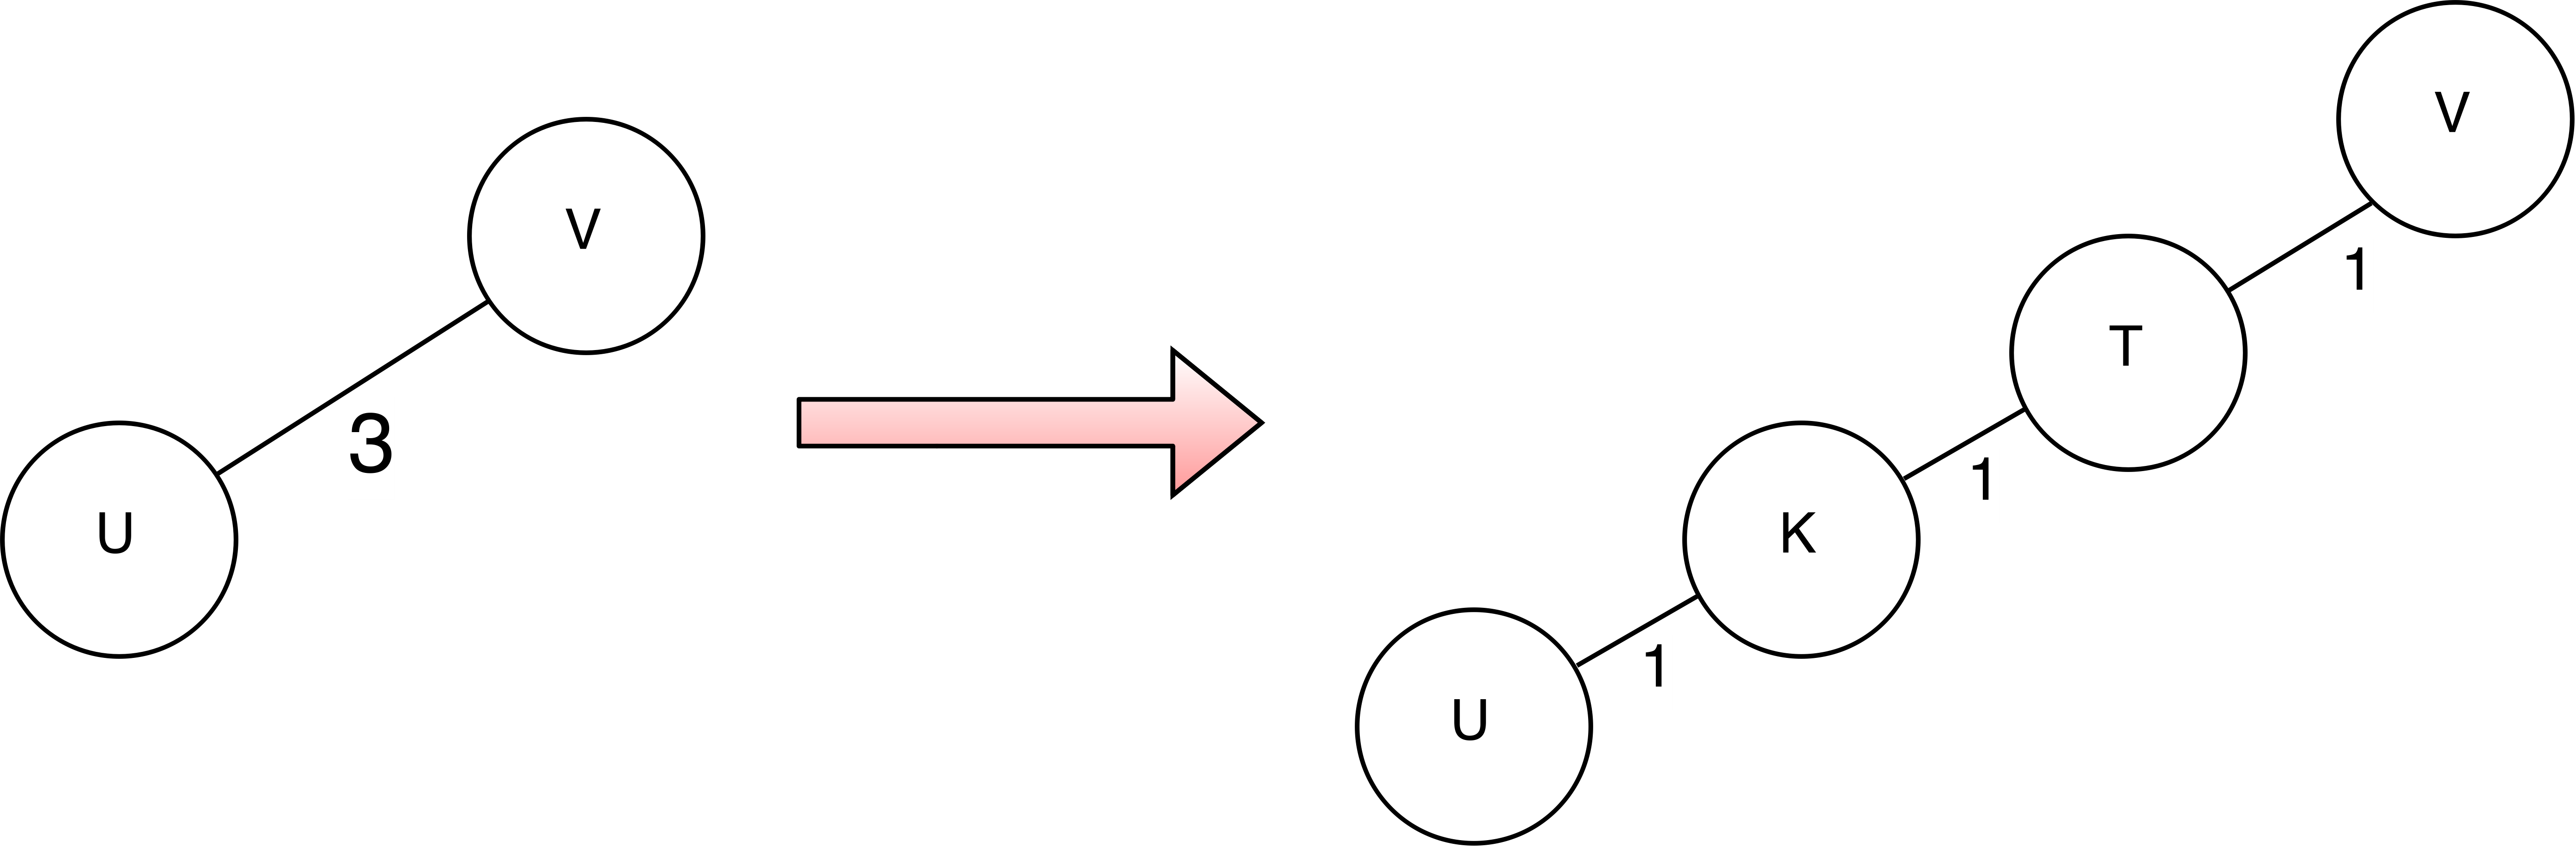
\includegraphics[width=0.9\textwidth]{img/floyd_social_modification.png}
\caption{Пример преобразования ребра}
\label{edge_modification}
\end{figure}
\FloatBarrier

В этой модификации алгоритм в худшем случае будет работать за $O(c \ VE)$ за счет увеличения числа ребер в $c$ раз.

